\documentclass[conference]{IEEEtran}

\usepackage[utf8]{inputenc}
\usepackage[T1]{fontenc}
\usepackage[brazil]{babel}
\usepackage{graphicx}
\usepackage{booktabs}
\usepackage{amsmath}
\usepackage{url}
\usepackage{xcolor}

\graphicspath{{imagens/}{../imagens/}}

\begin{document}

\title{RideSmart: Modelagem e Análise de Rotas\\ Urbanas com Grafos em Lagoa Nova, Natal/RN}

\author{\IEEEauthorblockN{Matheus Rodrigues Marinho}
\IEEEauthorblockA{Estrutura de Dados II (DCA3702, Unidade 3)\\
Universidade Federal do Rio Grande do Norte (UFRN)\\
Natal, Brasil}}

\maketitle

\begin{abstract}
Este trabalho modela a malha viária de Lagoa Nova (Natal/RN) como um grafo
direcionado e compara quatro algoritmos de caminhos mínimos (Dijkstra simples,
Dijkstra com heap, A* com heurística geográfica e Dijkstra bidirecional) sob três
funções de custo: distância, tempo sem trânsito e tempo com trânsito. O
congestionamento vem de um modelo sintético de dia típico, ancorado nas
avenidas reais do OpenStreetMap e modulado por um perfil que varia hora a hora. Além
de medir a eficiência de cada algoritmo, investigamos o problema do ponto de
embarque: vale a pena caminhar até um ponto $P$ perto da origem para reduzir o custo
total da viagem? Os resultados mostram o ganho expressivo do heap sobre a busca
linear, a economia de nós do A* e, principalmente, que o benefício de caminhar muda
conforme a função de custo e o horário.
\end{abstract}

\begin{IEEEkeywords}
grafos, caminhos mínimos, Dijkstra, A*, OSMnx, mobilidade urbana
\end{IEEEkeywords}

\section{Introdução}
Aplicativos de mobilidade urbana como Uber, 99 e Waze resolvem, no fundo, um problema
de caminho mínimo sobre a malha viária. Partindo dessa ideia, este projeto explora uma
variante prática: dados um ponto de origem $A$, um destino $B$ e uma distância máxima
de caminhada $X$, qual é o melhor ponto de embarque $P$? A rota completa tem dois
trechos: $A \rightarrow P$ a pé e $P \rightarrow B$ de carro.

Como estudo de caso, escolhemos o percurso entre a UFRN (Campus Central) e o
Midway Mall, em Natal/RN, com $X = 500$\,m. A meta não é apenas achar a rota
ótima, e sim comparar os algoritmos clássicos e entender como a escolha dos pesos e o
trânsito mudam a decisão.

\section{Modelagem do Problema}
A rede viária foi obtida do OpenStreetMap com a biblioteca OSMnx~\cite{boeing2017}. O
grafo é um MultiDiGraph $G=(V,E)$ com $|V|=3374$ nós e $|E|=8014$ arestas,
cobrindo um raio de 3\,km em torno do ponto central. Os nós são interseções e
extremidades de vias; as arestas são segmentos de rua, e o grafo preserva mão
única e vias paralelas. A Fig.~\ref{fig:rede} mostra a malha completa.

\begin{figure}[!t]
\centering
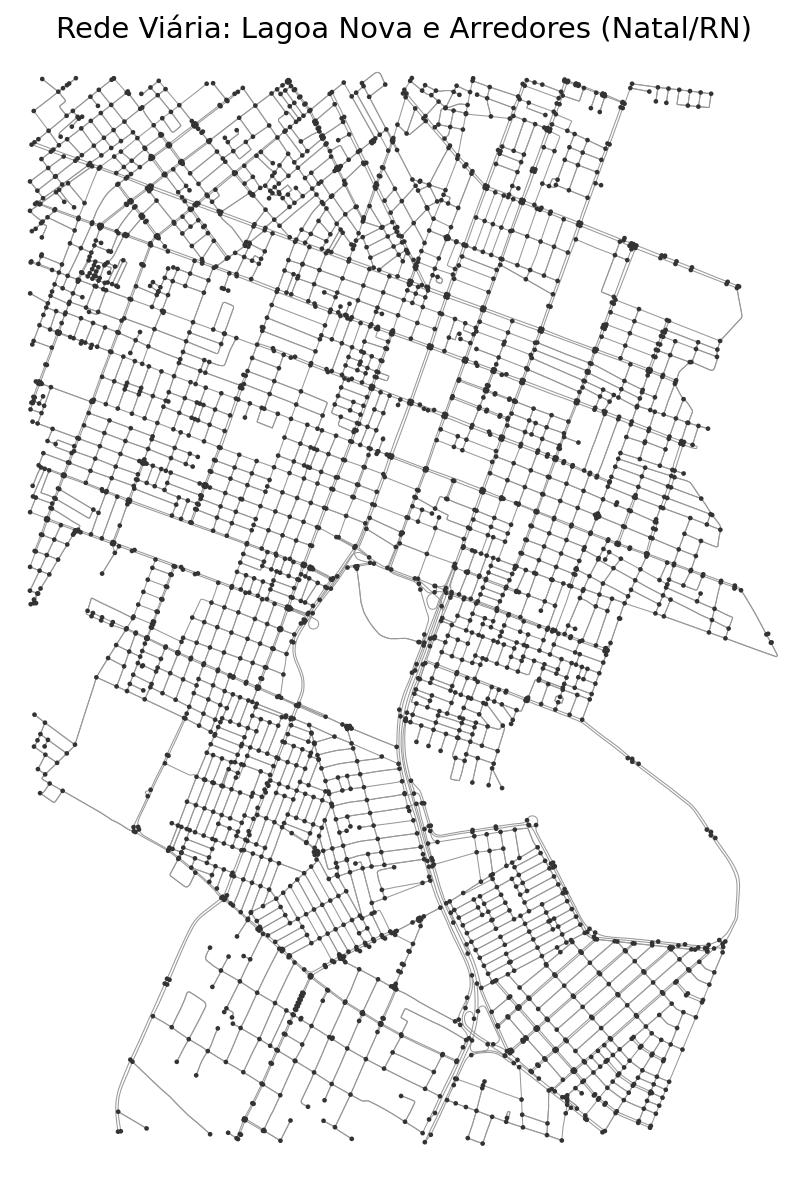
\includegraphics[width=\columnwidth]{01_rede_completa.png}
\caption{Rede viária de Lagoa Nova e arredores (Natal/RN) extraída do OpenStreetMap.}
\label{fig:rede}
\end{figure}

\subsection{Funções de custo}
Definimos três funções de peso para as arestas:
\begin{itemize}
 \item Distância (\texttt{length}): comprimento do segmento em metros;
 \item Tempo sem trânsito (\texttt{travel\_time}): calculado a partir da
 velocidade da via informada pelo OSM;
 \item Tempo com trânsito (\texttt{travel\_time\_traffic}): o tempo livre
 penalizado por um fator de congestionamento sintético.
\end{itemize}

\subsection{Trânsito sintético: um ``dia típico''}
Em vez de penalizar arestas ao acaso, ancoramos o congestionamento na geometria real e
o modulamos pelo horário, cruzando dois eixos:
\begin{itemize}
 \item Onde (espacial): a hierarquia viária (avenidas saturam mais que ruas
 residenciais) e os corredores arteriais reais, identificados pelo nome no
 OSM. A Av. Senador Salgado Filho se destaca, por ser a via com mais arestas
 arteriais na área (no total, 754 arestas pertencem aos 8 corredores escolhidos);
 \item Quando (temporal): um perfil de intensidade $I(h)\in[0,1]$ ao longo do
 dia, bimodal (pico de manhã, repique no almoço e o pico mais forte por volta das
 18\,h; de madrugada o trânsito é quase livre).
\end{itemize}
O fator de congestionamento de cada aresta no horário $h$ é
\begin{equation}
\text{fator}(h) = 1 + \text{inc}_{\text{base}} \cdot I(h) \cdot \varepsilon,
\end{equation}
em que $\text{inc}_{\text{base}}$ é a severidade espacial (hierarquia vezes o reforço de
corredor) e $\varepsilon$ é um ruído de $\pm10\%$ que simula incidentes pontuais. As
Fig.~\ref{fig:perfil} e~\ref{fig:horarios} mostram, respectivamente, o perfil ao longo
do dia e a malha colorida pelo congestionamento em quatro horários. Vale deixar claro
que tratamos esse perfil como o de um dia útil comum: é uma simplificação consciente, já
que não usamos dados reais de fluxo medido.

\begin{figure}[!t]
\centering
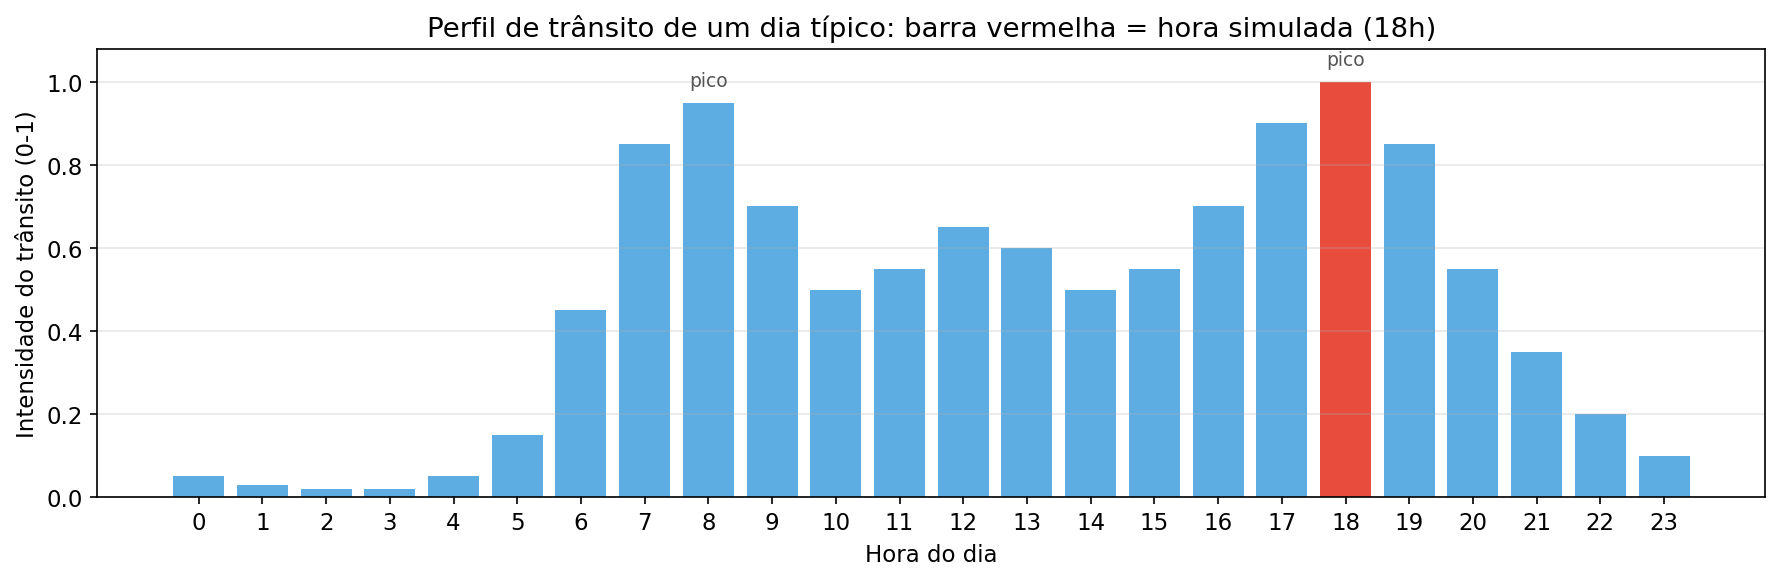
\includegraphics[width=\columnwidth]{06_perfil_horario.png}
\caption{Perfil de intensidade do trânsito ao longo de um dia típico. A hora simulada
(18\,h) está destacada.}
\label{fig:perfil}
\end{figure}

\begin{figure}[!t]
\centering
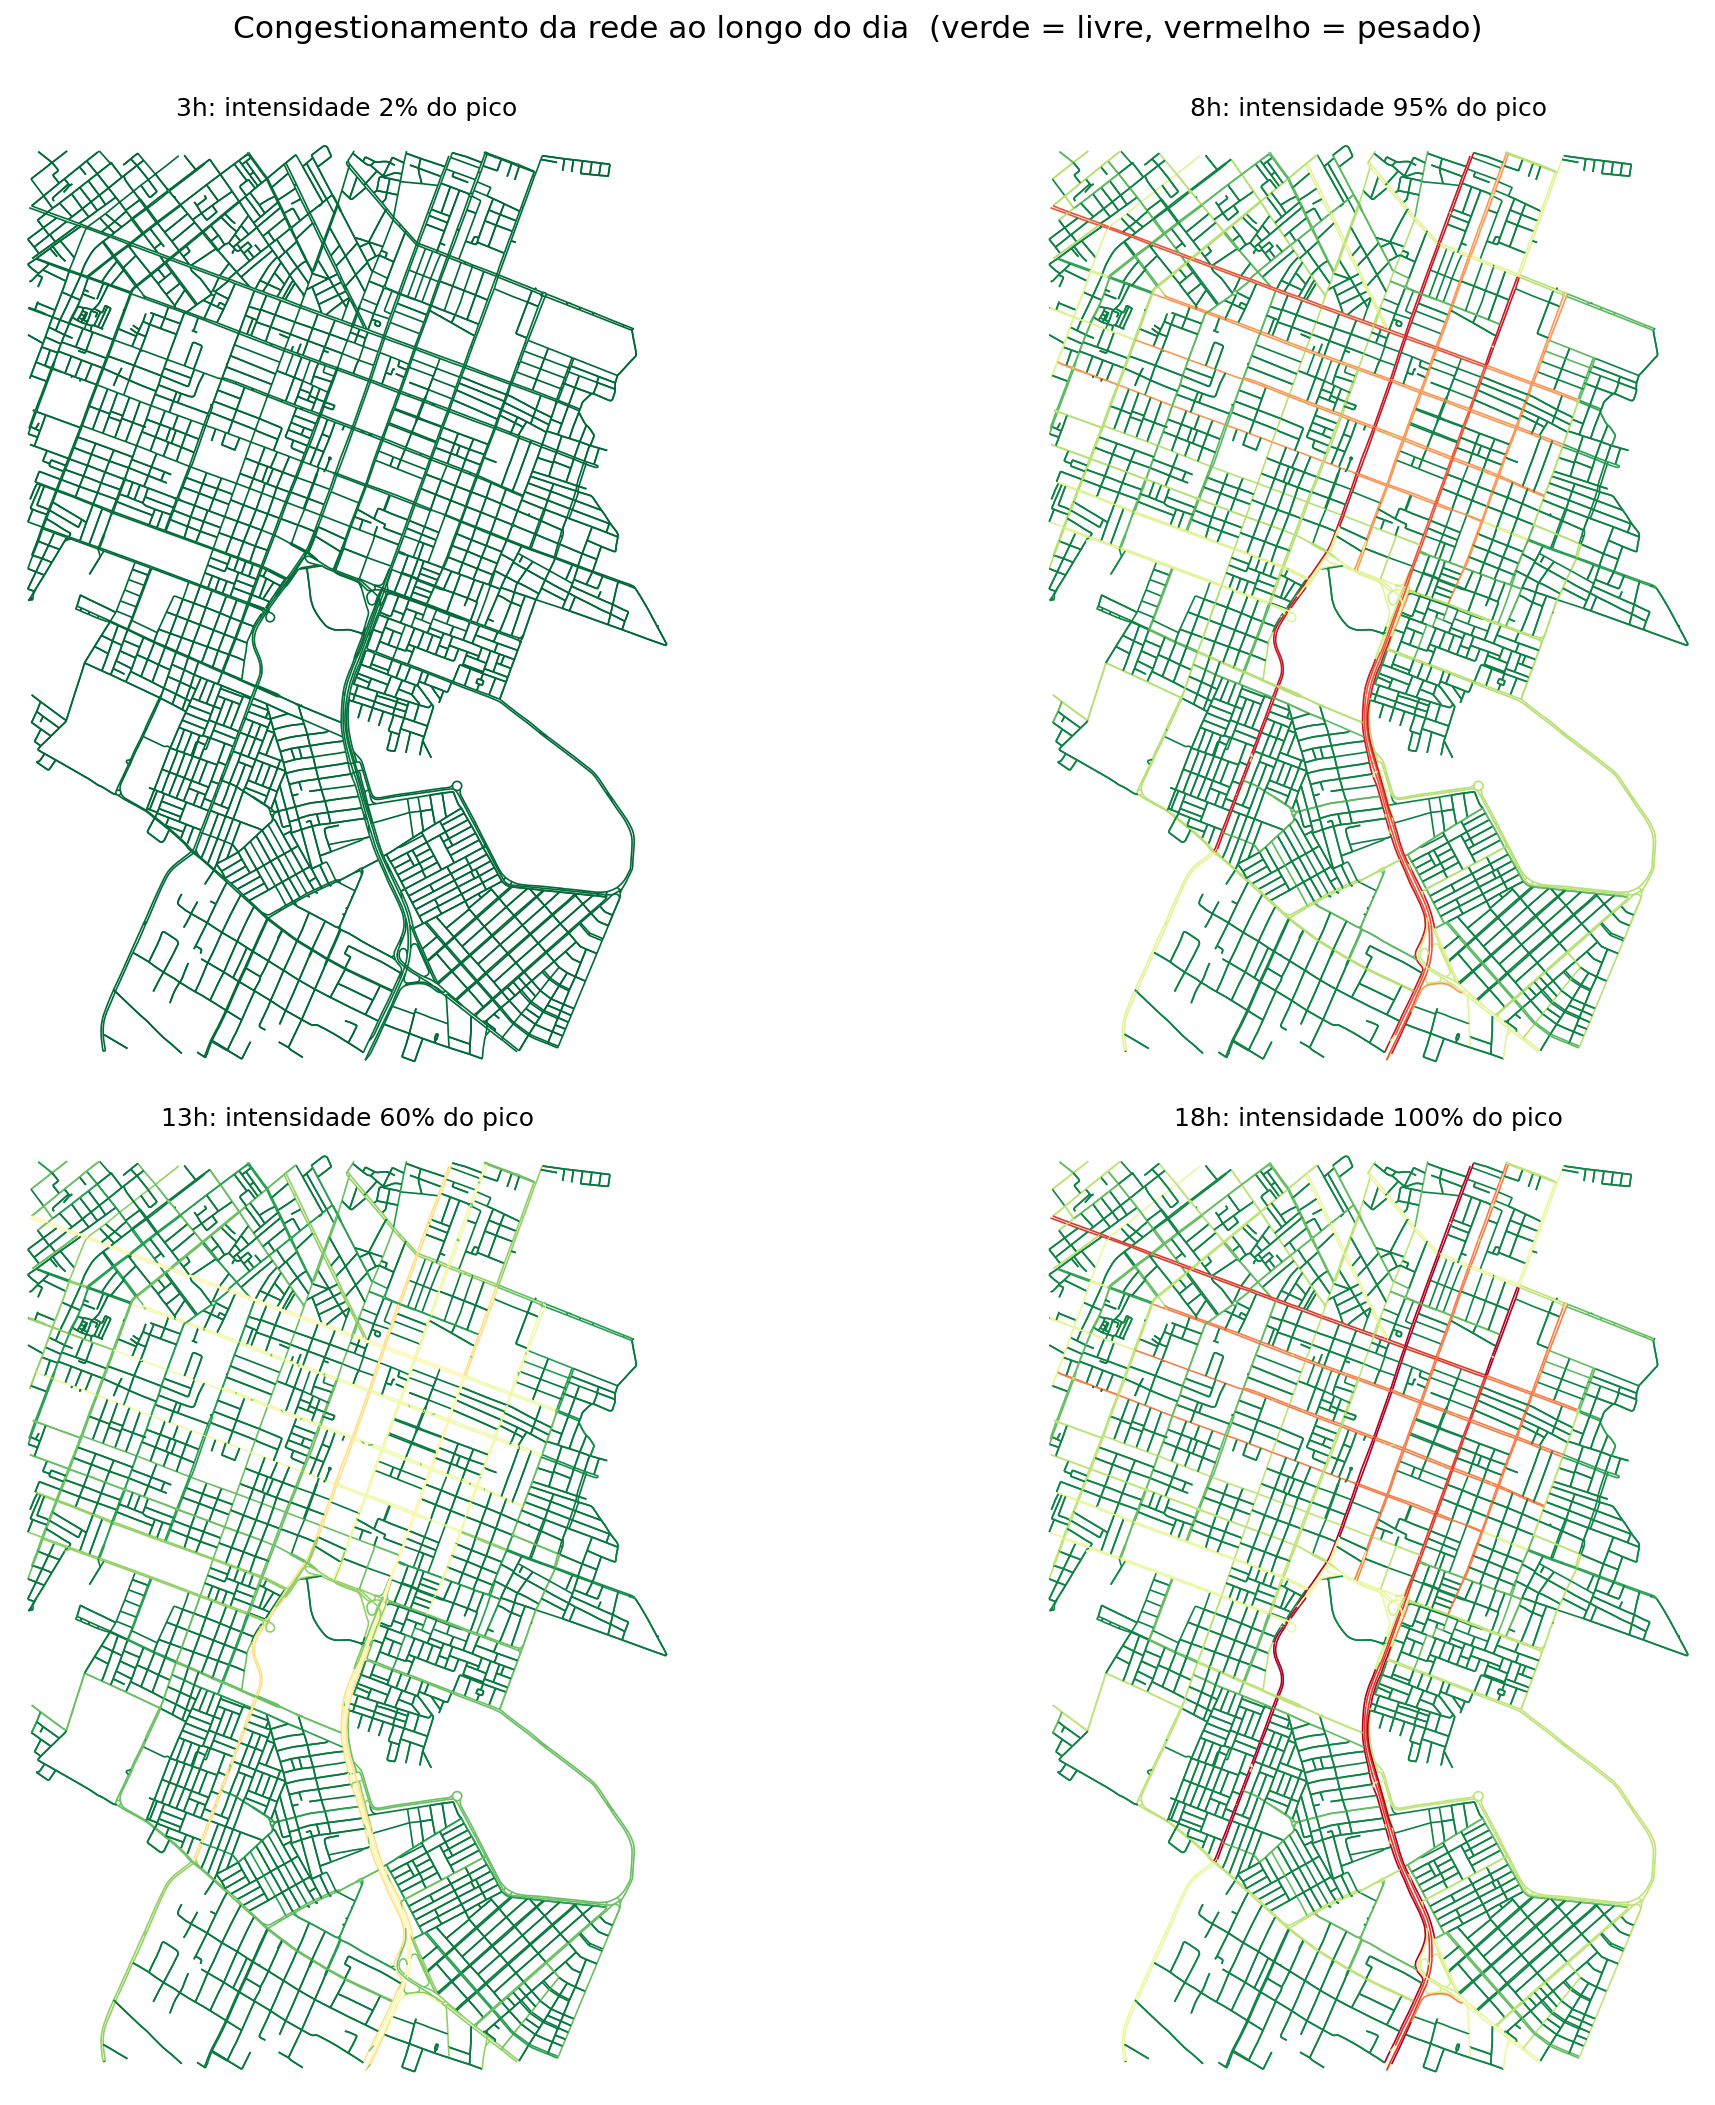
\includegraphics[width=\columnwidth]{07_comparacao_horarios.png}
\caption{Congestionamento da rede em quatro horários (escala de cor fixa). Os corredores
arteriais ``acendem'' no pico das 18\,h.}
\label{fig:horarios}
\end{figure}

\section{Algoritmos Utilizados}
Implementamos todos os algoritmos do zero (sem usar
\texttt{networkx.shortest\_path}); cada um devolve a tripla
(caminho, custo, nós expandidos).

\begin{itemize}
 \item Dijkstra simples~\cite{dijkstra1959}: faz busca linear pelo nó não
 visitado de menor distância. Tem complexidade $O(V^2)$ e serve de baseline.
 \item Dijkstra com heap: usa uma fila de prioridade (heap binário) para
 extrair o mínimo em $O(\log V)$, chegando a $O((V+E)\log V)$.
 \item A*~\cite{hart1968}: usa $f(n)=g(n)+h(n)$ com heurística haversine
 (distância geodésica). Ela é admissível, pois nunca superestima o custo real.
 \item Dijkstra bidirecional: o algoritmo adicional da literatura. Roda duas
 buscas ao mesmo tempo (uma da origem para frente e outra do destino para trás), que se
 encontram no meio e reduzem o espaço explorado.
\end{itemize}

\section{Experimentos}
Rodamos os quatro algoritmos para as três funções de custo na rota direta
$A \rightarrow B$, com o trânsito fixado em 18\,h (horário de pico). Em cada execução
medimos o custo total, o número de nós expandidos e o tempo de execução. Depois, para a
análise do ponto de embarque, levantamos todos os nós a até 500\,m de caminhada de $A$
(29 candidatos $P$) e, para cada função de custo, escolhemos o $P$ que minimiza o custo
total $A \rightarrow P \rightarrow B$.

\section{Resultados}

\subsection{Eficiência dos algoritmos}
A Tabela~\ref{tab:algos} resume os resultados para o peso distância. Os quatro
algoritmos chegaram ao mesmo caminho ótimo (custo idêntico), o que confirma que
as implementações estão corretas; a diferença aparece só na eficiência.

\begin{table}[!t]
\caption{Rota direta $A\rightarrow B$ por distância (custo = 5795{,}24\,m).}
\label{tab:algos}
\centering
\begin{tabular}{lrr}
\toprule
Algoritmo & Nós expandidos & Tempo (ms) \\
\midrule
Dijkstra Simples & 2365 & 364{,}9 \\
Dijkstra com Heap & 2366 & 5{,}7 \\
A* & 1053 & 6{,}4 \\
Dijkstra Bidirecional & 2357 & 5{,}7 \\
\bottomrule
\end{tabular}
\end{table}

Dois pontos chamam a atenção (Fig.~\ref{fig:nos} e~\ref{fig:tempo}):
\begin{enumerate}
 \item O Dijkstra simples é cerca de 50 vezes mais lento
 ($\approx$365\,ms contra $\approx$6\,ms), mesmo expandindo o mesmo número de nós que a
 versão com heap. Na prática, isso mostra que quem manda no desempenho é a
 estrutura de dados, e não o algoritmo em si.
 \item O A* expande quase metade dos nós (1053 contra 2366), porque a
 heurística geográfica empurra a busca na direção do destino; o ganho em tempo é pequeno,
 já que calcular a heurística custa um pouco a cada nó.
\end{enumerate}

\begin{figure}[!t]
\centering
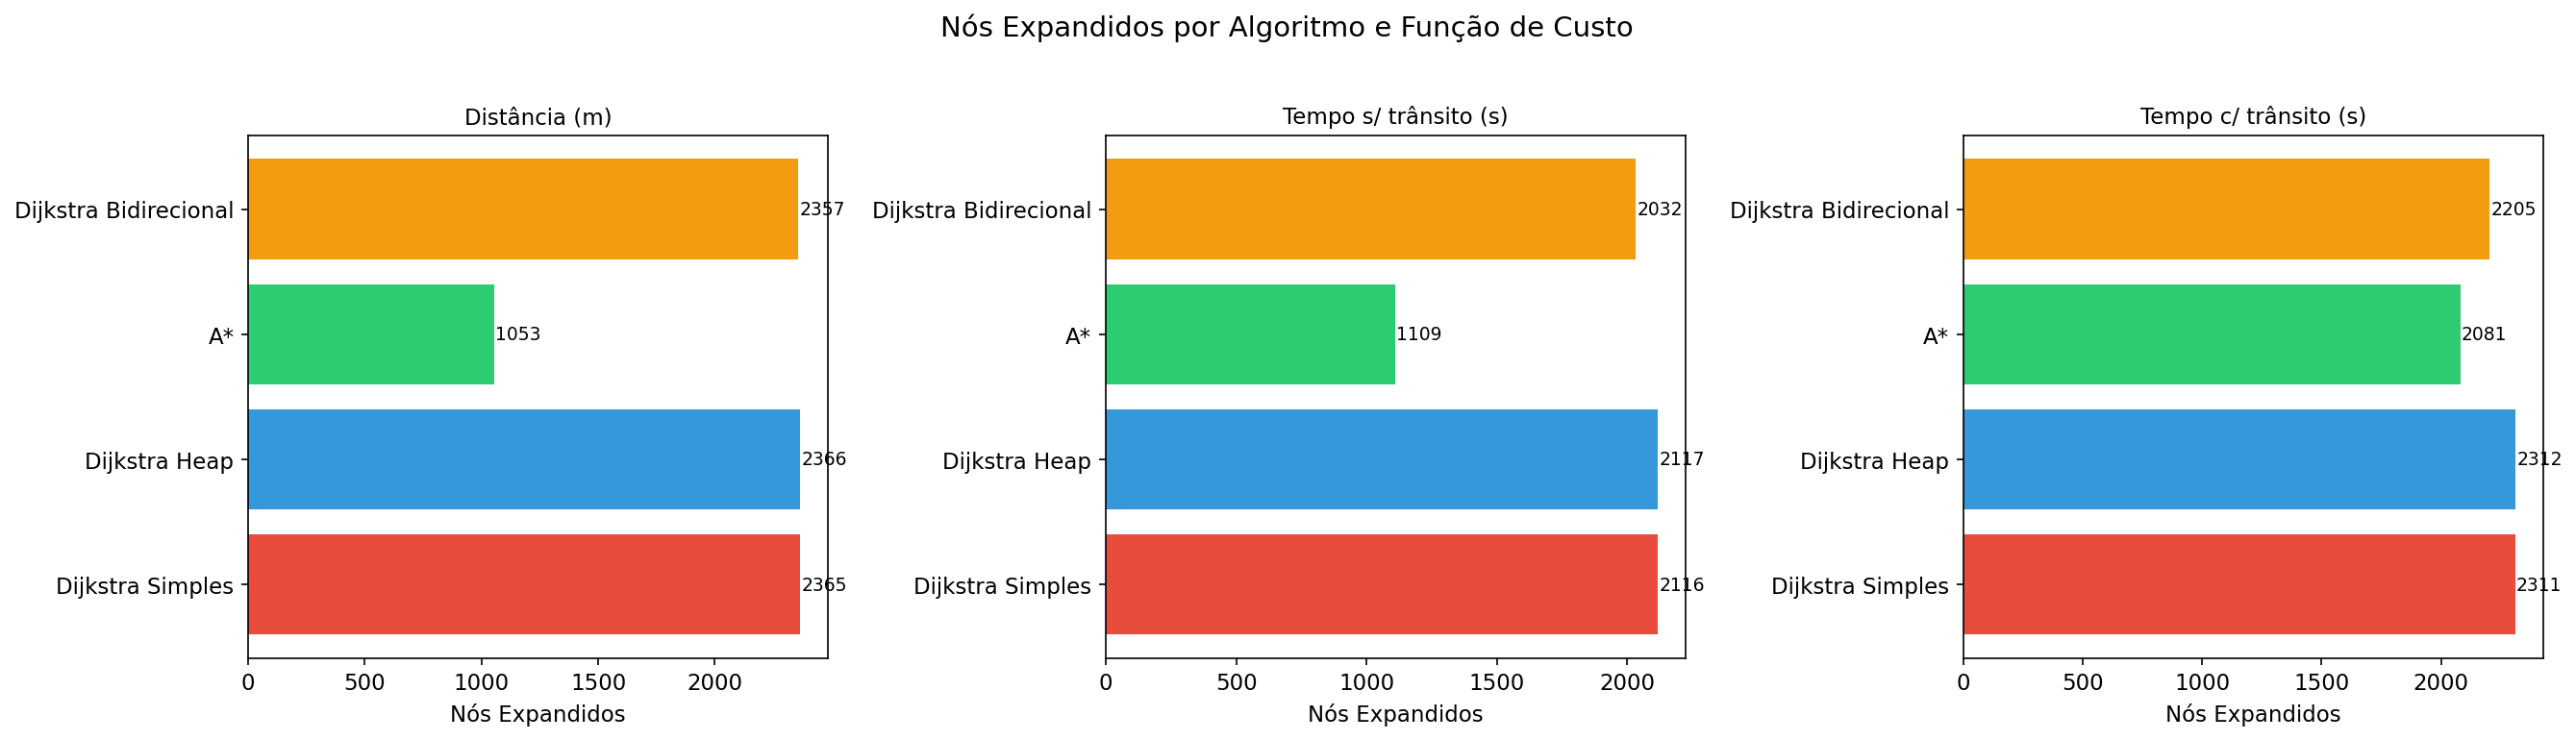
\includegraphics[width=\columnwidth]{02_nos_expandidos.png}
\caption{Nós expandidos por algoritmo e função de custo.}
\label{fig:nos}
\end{figure}

\begin{figure}[!t]
\centering
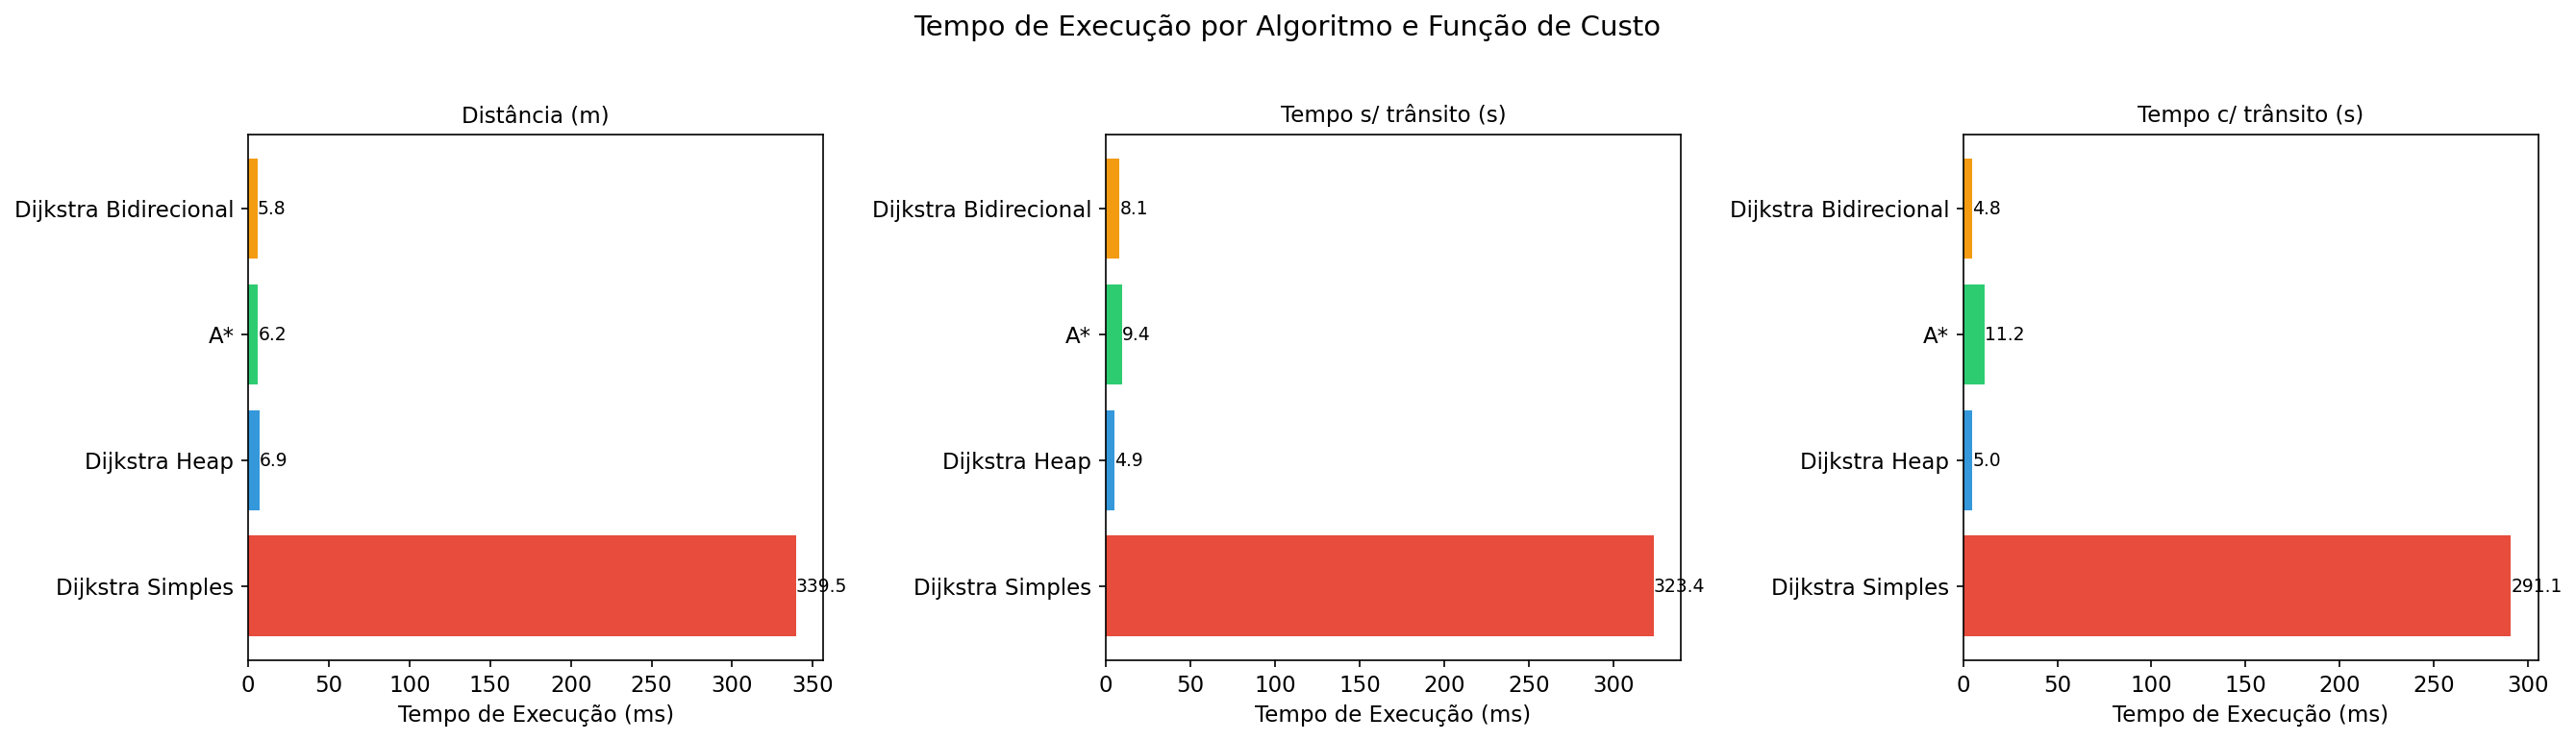
\includegraphics[width=\columnwidth]{03_tempo_execucao.png}
\caption{Tempo de execução por algoritmo e função de custo.}
\label{fig:tempo}
\end{figure}

\subsection{Impacto dos pesos e do ponto de embarque}
A Tabela~\ref{tab:walk} compara a rota direta com a melhor rota que passa por um ponto de
embarque $P$. O efeito depende do critério:
\begin{itemize}
 \item Em distância, caminhar 329\,m até $P$ encurtou o percurso em
 5{,}7\%;
 \item Em tempo sem trânsito, o desvio não compensou ($-1{,}8\%$);
 \item Em tempo com trânsito (18\,h), nenhum ponto dentro de 500\,m da origem
 analisada bateu a rota direta ($-5{,}2\%$): o tempo a mais de caminhada não pagou o
 alívio do congestionamento.
\end{itemize}
Ou seja, caminhar até outro ponto não é uma regra geral; o resultado depende da
topologia, do critério e do horário.

\begin{table}[!t]
\caption{Rota direta vs. rota com caminhada (melhor $P$).}
\label{tab:walk}
\centering
\begin{tabular}{lrrr}
\toprule
Função de custo & Direto & Via $P$ & Ganho \\
\midrule
Distância (m) & 5795{,}2 & 5463{,}2 & $+5{,}7\%$ \\
Tempo s/ trânsito (s) & 380{,}8 & 387{,}7 & $-1{,}8\%$ \\
Tempo c/ trânsito (s) & 730{,}6 & 768{,}3 & $-5{,}2\%$ \\
\bottomrule
\end{tabular}
\end{table}

\section{Discussão Crítica}
A menor distância nem sempre é a rota mais rápida: avenidas mais longas, porém
mais velozes, podem ganhar de atalhos por ruas residenciais. Como o trânsito penaliza os
corredores arteriais, no pico o algoritmo desvia para vias secundárias, um comportamento
parecido com o que se vê na cidade.

Entre os algoritmos, o Dijkstra com heap é a melhor escolha de uso geral: é
rápido, estável e funciona bem com qualquer peso. O A* leva vantagem em nós
expandidos, mas isso depende da qualidade da heurística, que perde força no cenário com
trânsito, já que a estimativa pela velocidade livre subestima o tempo real. O
bidirecional compensa em grafos grandes, ao custo de uma implementação mais
complicada.

As principais limitações são: (i) o trânsito, ainda que ancorado em vias reais,
é sintético e calibrado à mão; (ii) as velocidades do OSM nem sempre são precisas;
(iii) a caminhada usa a rede de carros, ignorando calçadas e atalhos de pedestres; e
(iv) o grafo é estático. Como próximos passos, o modelo poderia usar dados reais
de trânsito (APIs de mobilidade), uma rede de pedestres própria e
predição de congestionamento com aprendizado de máquina.

\section{Conclusão}
Este trabalho aplicou algoritmos de caminhos mínimos a um problema real de mobilidade em
Lagoa Nova, Natal/RN. Os experimentos deixaram claro o peso da estrutura de dados (o heap
foi cerca de 50 vezes mais rápido que a busca linear) e a economia de nós que o A*
proporciona. Também ficou evidente que a escolha dos pesos e o horário de pico mudam
bastante a rota e o quanto vale a pena caminhar até um ponto de embarque alternativo, um
trade-off que precisa ser pensado caso a caso. No fim, temos uma base simples, mas
fiel à cidade, para raciocinar sobre decisões de roteamento urbano.

\begin{thebibliography}{1}
\bibitem{dijkstra1959} E. W. Dijkstra, ``A note on two problems in connexion with
graphs,'' Numerische Mathematik, vol. 1, pp. 269-271, 1959.
\bibitem{hart1968} P. E. Hart, N. J. Nilsson e B. Raphael, ``A formal basis for the
heuristic determination of minimum cost paths,'' IEEE Trans. Syst. Sci. Cybern.,
vol. 4, no. 2, pp. 100-107, 1968.
\bibitem{boeing2017} G. Boeing, ``OSMnx: New methods for acquiring, constructing,
analyzing, and visualizing complex street networks,'' Computers, Environment and
Urban Systems, vol. 65, pp. 126-139, 2017.
\end{thebibliography}

\end{document}
